\chapter{مقدمه}

\section{مقدمه}
با پیشرفت روزافزون دانش بشری در دهه اخیر و تلفیق هرچه بیشتر شاخه های علمی با یکدیگر و همچنین همگام شدن و بهره‌مندی از فناوری های موجود شاهد ساخته شدن محصولات جدیدی هستیم که ربات‌ها یکی از معروف و محبوب ترین این محصولات می‌باشند.

%در دهه‌های اخیر، پیشرفت‌های چشمگیری در زمینه‌ی رباتیک و هوش مصنوعی به وجود آمده است که منجر به ایجاد روش‌ها و تکنیک‌های نوین برای طراحی و کنترل ربات‌ها گردیده است.%
در این پایان‌نامه، به اختصار به طراحی و پیاده‌سازی ربات چهارپای عنکبوتی را که ساخته شده است اشاره شده و سپس به تفصیل درباره انتخاب و کالیبره‌سازی دوربین، نحوه ارتباطات بین قطعات الکترونیکی و مکانیکی،الگوریتم تشخیص موانع و نحوه‌ی اجرای و ارزیابی آزمایش‌ها خواهیم پرداخت. همچنین، نتایج و تحلیل‌های حاصل از آزمایش‌ها به منظور ارزیابی کارایی و کاربردی بودن این روش در محیط‌های واقعی را ارائه خواهیم داد.

در انتها نیز به بررسی چالش های پیاده سازی پرداخته و پیشنهاداتی برای کارهای آینده خواهیم پرداخت.


\section{ربات و انواع آن}

\subsection{ربات‌های سری}
بطور معمول ربات‌ها با توجه به نوع كاربردشان، به شكل سري، موازي و يا تركيبي از هر دو ساخته مي‌شوند. همان طور كه در شكل
\ref{ربات سریال}
نشان داده شده است، رباتهاي سري از يك زنجيره
سينماتيكي تشكيل شده اند كه در آن مفاصل‌ در يك ارتباط سري باهم قرار مي‌گيرند. اين ربات‌ها به دليل ويژگي داشتن فضاي كاري بزرگتر در صنعت بسيار پرکاربرد هستند.
در این ربات‌ها معمولا عملگر
\noindent\unskip\LTRfootnote{َActuator}
ها با قرار گرفتن به صورت سري در هر مفصل قرار یک درجه آزادی ایجاد می‌کنند.
علارغم مزیت‌های ذکر شده برای این دسته از ربات ها باید توجه داشت که رباتهاي سري لزوماً براي تمامي کاربرد‌های صنعتي و حتی غير صنعتي، بهترين انتخاب نبوده و معایبی نیز به همراه دارند. از جمله این معایب آنکه خطاهاي موقعيتي در آنها جمع شونده هستند. از ديدگاه انرژي ميزان مصرف انرژي در اين ربات‌ها بالا است؛ زيرا هر كدام از
مفاصل تحريك‌شده نه تنها بار را حمل مي‌كنند بلكه بايد بازوها ماقبل خود را نيز جابه‌جا نمايد. در نتيجه براي جابه‌جايي بارهاي سنگين بازوهاي قوي تري مورد نياز است. در رباتهاي سري تمامي مفاصل بايد كار كنند، اگر يك مفصل از كار بيافتد يا آزاد گذاشته شود ساختار ربات به هم ریخته و در اين حالت ربات قادر به حفظ موقعيت خود و انجام وظیفه
\noindent\unskip\LTRfootnote{Task}
محوله نخواهد بود.


\begin{figure}[H]
	\centering
	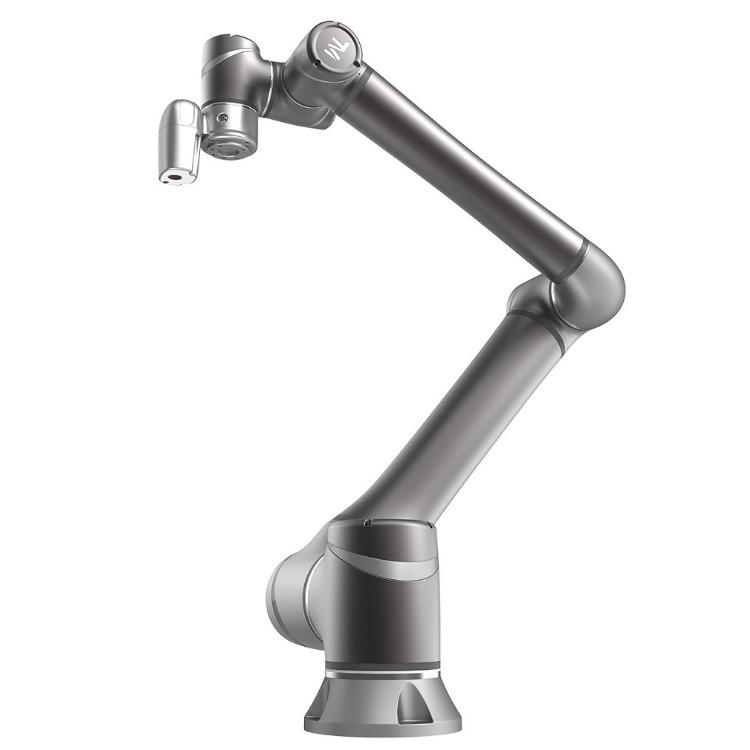
\includegraphics[width=0.5\textwidth]{./images/Chapter1/TechmanTM12}	
	\caption[ربات سری]{ربات سری \cite{SerialRobot}}
	\label{ربات سریال}
\end{figure}
\noindent
\unskip

\subsection{ربات‌های موازی}

به مرور زمان احساس نیاز به ســاختارهايي كه محدوديت‌هاي ربات‌های سـری را نداشـته باشند به وجود آمد. همانگونه كه ما انسان‌ها براي حركتهاي دقيق و يا برداشتن اجسام سنگين از هر دو دست خود استفاده مي‌كنيم، مي‌توان چنين تصـور كرد كه اسـتفاده از زنجيره‌هاي سـينماتيكي بسته كه چند بازو باهم و به صـورت موازي در حركت دخيل باشـند مي‌توانند پاسخي درخور براي اين مشكل باشد. 

همانطور که در شکل
\ref{ربات موازی}
مشاهده می‌شود ربات‌های موازي از زنجيره‌های بسـته سـينماتيكي سـاخته مي‌شوند كه شامل يك تكيه‌گاه
\noindent\unskip\LTRfootnote{Base}
و يك صفحه متحرك
\noindent\unskip\LTRfootnote{Moving Platform}
كه به وسيله تعدادي عملگر يا رابط به يكديگر متصل شده اند، مي باشد. مهمترين ضعف رباتهاي موازي محدوديت در فضاي كاری آنهاست. 
\begin{figure}[H]
	\centering
	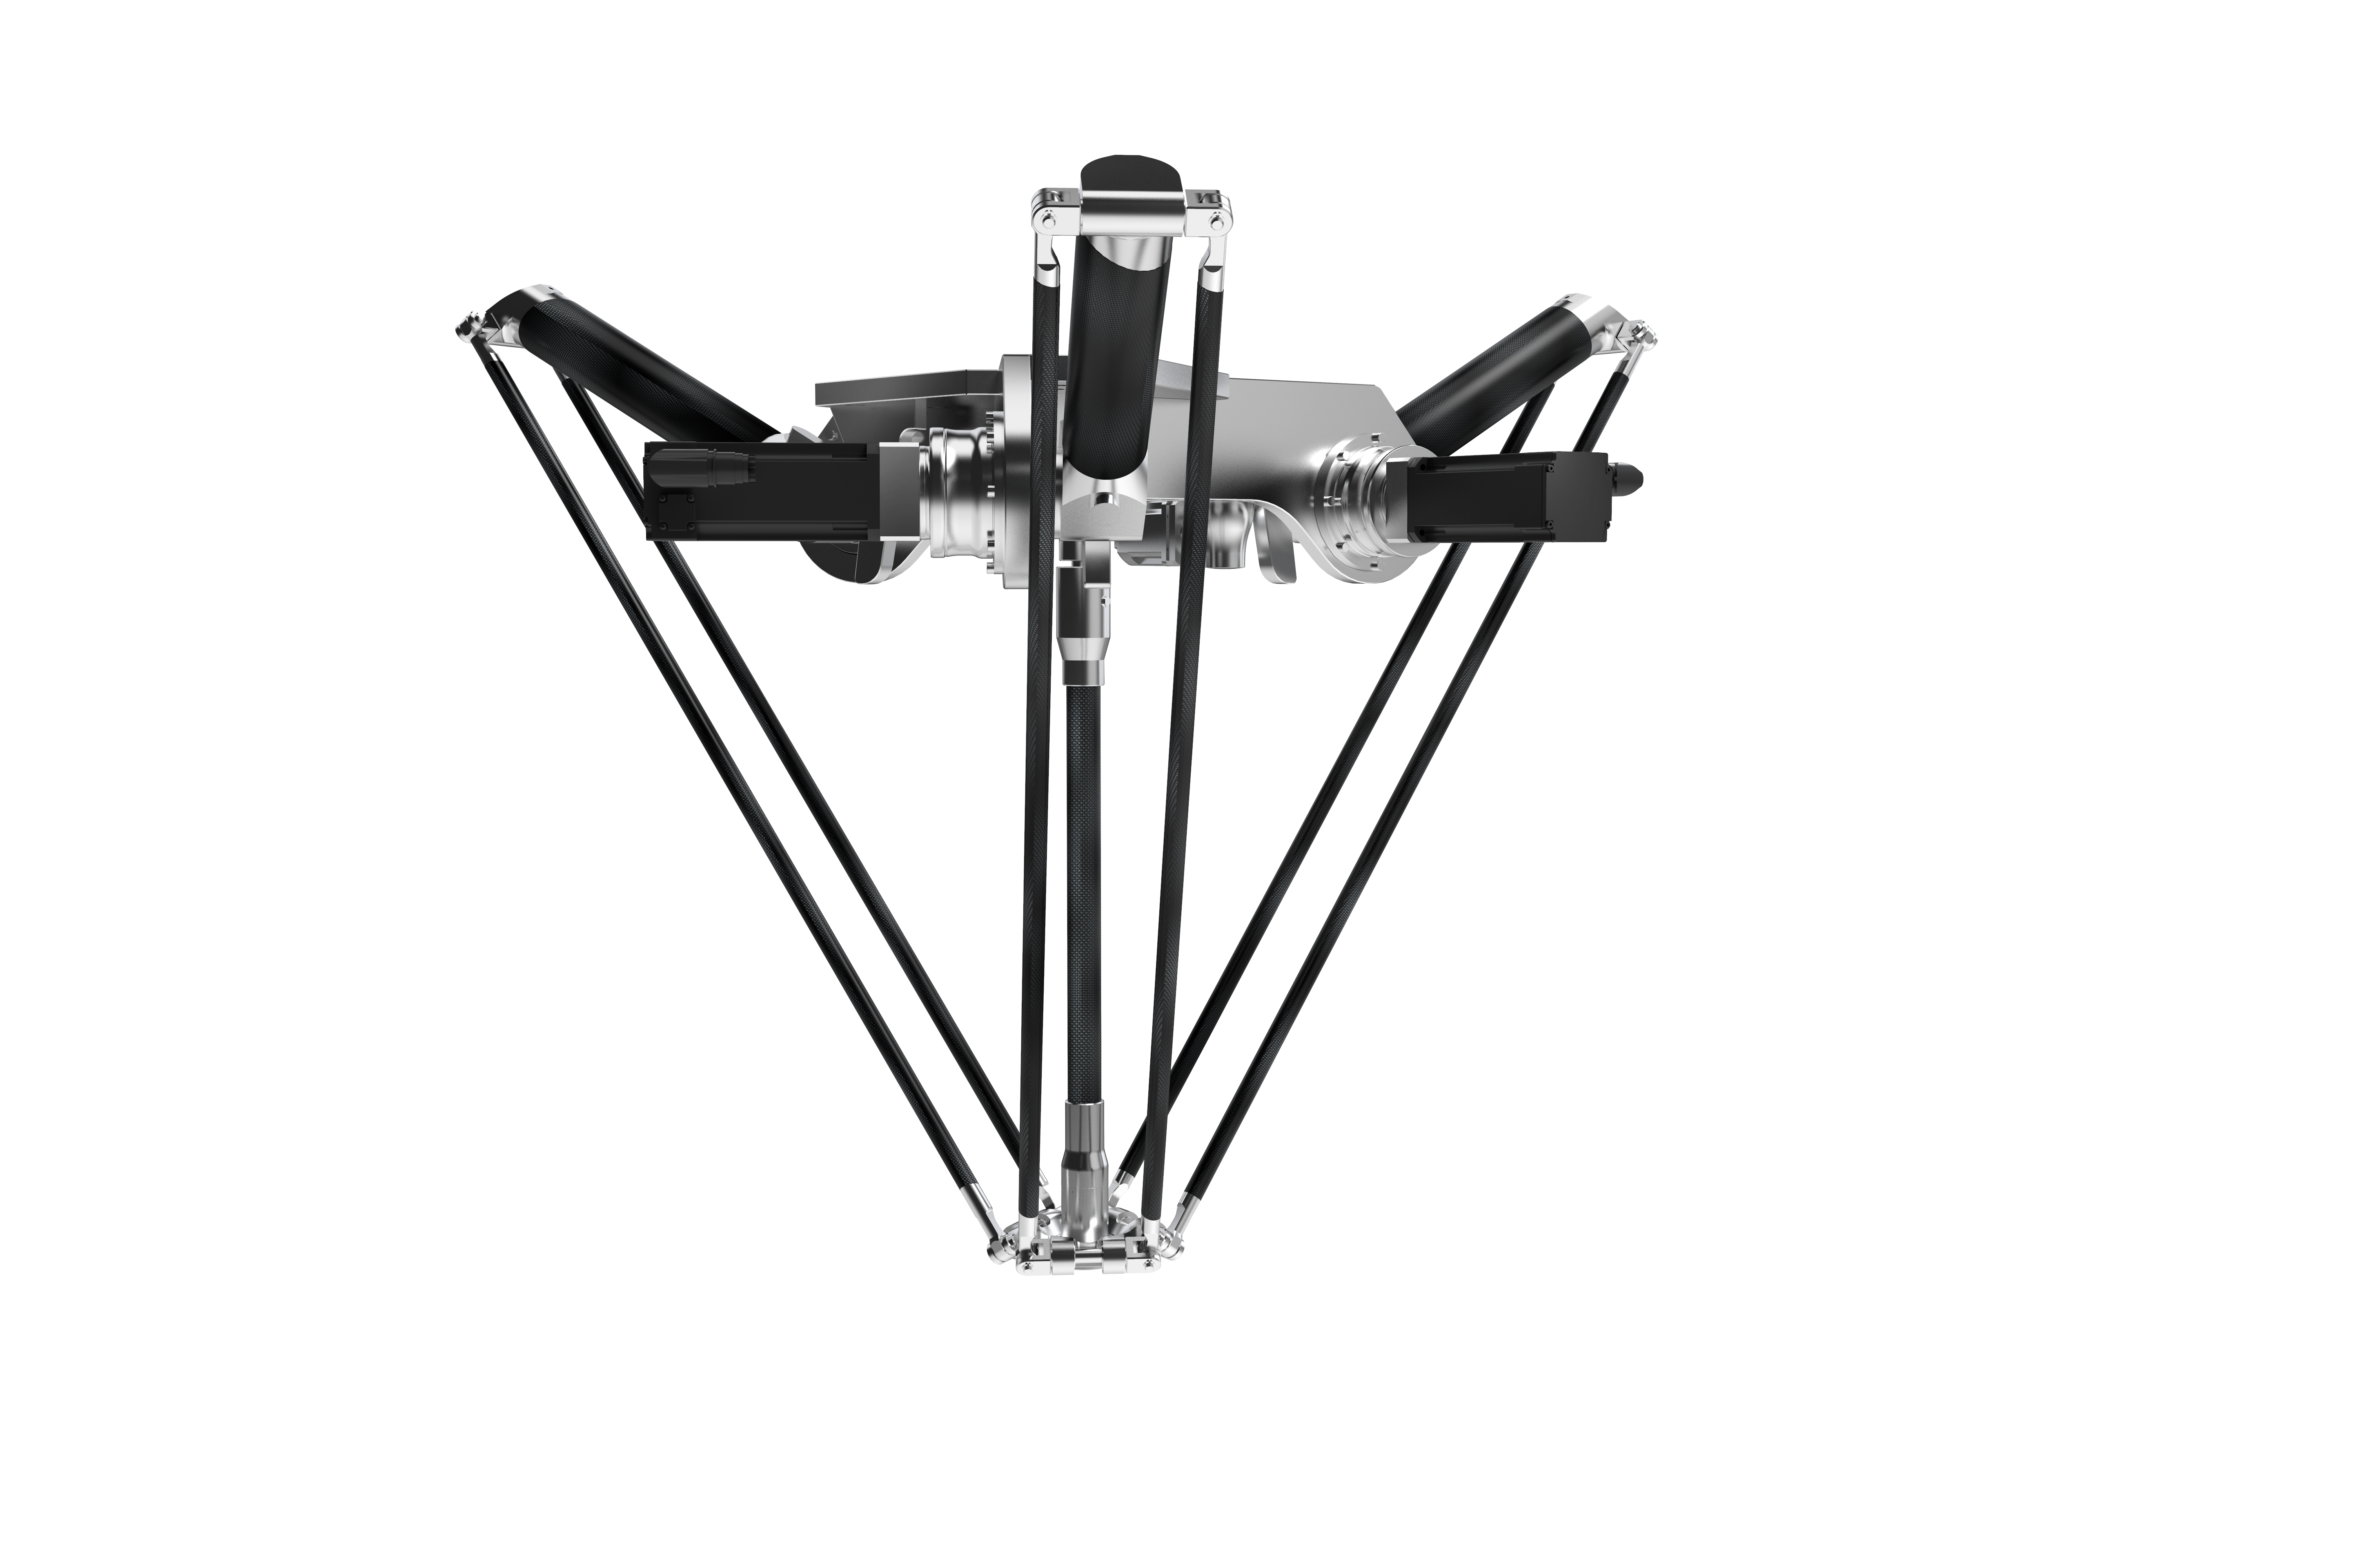
\includegraphics[width=0.5\textwidth]{./images/Chapter1/Delta2}	
	\caption[ربات موازی]{ربات موازی \cite{ParallelRobot}}
	\label{ربات موازی}
\end{figure}
\noindent
\unskip


\subsection{ربات‌های متحرک}
در دهه‌های اخیر، ربات‌های متحرک
\noindent\unskip\LTRfootnote{Mobile Robots}
به عنوان به عنوان ابزاری چندمنظوره و قدرتمند در دنیای مدرن از ماشین‌های خودکار تلقی می‌شوند. ربات‌های متحرک، از جمله دستاوردهای بزرگ در زمینه‌های مختلف از تحقیقات تا کاربردهای عملی، توانسته‌اند نقش مهمی را ایفا کنند. از تعقیب کاربردهای صنعتی تا خدمات انسانی و حتی مسائل محیط‌زیستی، علیرغم تنوع گسترده‌ی شکل‌ها و ساختارها، ربات‌های متحرک، توانایی انجام وظایف متنوع در محیط‌های مختلفی مانند صنایع کشاورزی، خدماتی و... را دارا هستند.
\begin{figure}[H]
	\centering
	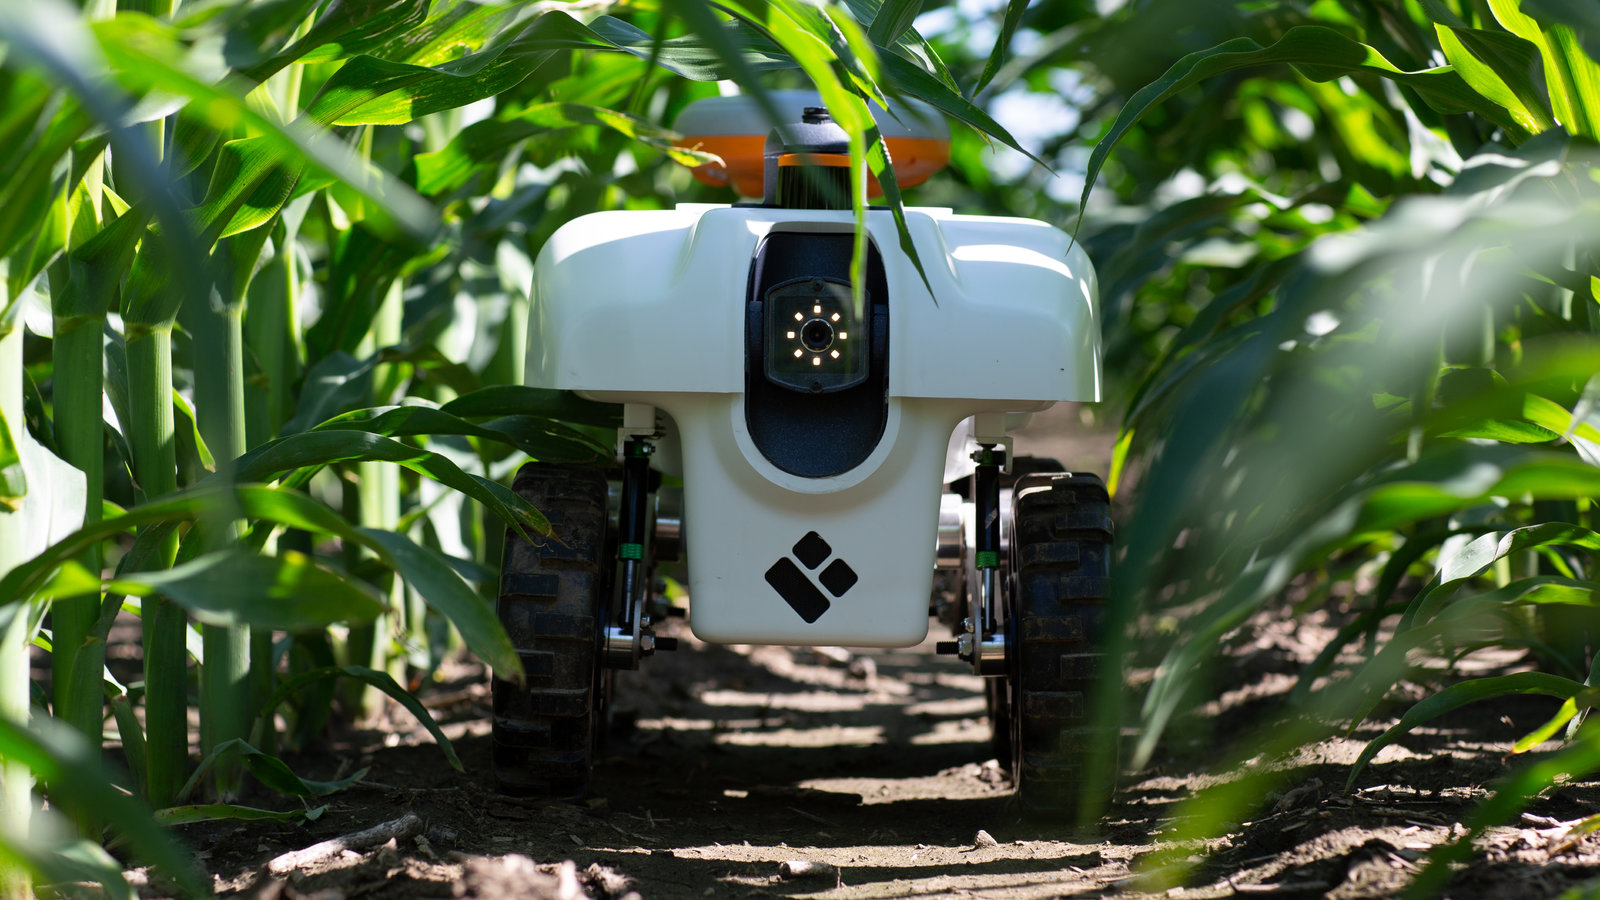
\includegraphics[width=0.5\textwidth]{./images/Chapter1/AgRobot}	
	\caption[ربات کشاورزی]{ربات کشاورزی \cite{AgRobot}}
	\label{ربات کشاورزی}
\end{figure}
\noindent
\unskip

ربات‌های متحرک در انواع مختلف طراحی می‌شوند که هر یک برای انجام وظایف خاصی از مکانیزم‌های متمایز استفاده می‌کنند. ربات‌های چرخدار
\noindent\unskip\LTRfootnote{Wheeled Robots}
، به عنوان مثال، از چرخ‌های محرک دارای موتورها برای حرکت و جابجایی استفاده می‌کنند. اینگونه ربات‌ها از استیکرهای تفاضلی بهره می‌برند که چرخ‌های موتورها در سمت‌های مختلف با سرعت‌های متفاوت می‌چرخند تا امکان تغییر جهت را فراهم کنند. 
ربات‌های پادار
\noindent\unskip\LTRfootnote{Legged Robots}
تلاش می‌کنند تا حرکت حیوانات را تقلید کنند و از پاها برای حرکت استفاده می‌کنند. کنترل ربات‌های پاهادار به دلیل درجات آزادی متعدد در مفاصل پیچیده‌است. ربات‌های هوایی مانند پهپادها، با استفاده از پره‌ها برای تولید لیفت و تراکم برای پرواز بهره می‌برند. این ربات‌ها نیاز به الگوریتم‌های کنترل پیچیده دارند تا پایداری و مسیر طی‌شده را مدیریت کنند.
\cite{Craig}

\section{ربات عنکبوتی چهارپا}
\subsection{ربات‌های عنکبوتی}
راه رفتن با چهار پا برای اکثر حیوانات رایج است و دلیل خوبی برای تکرار آن در ربات‌ها وجود دارد. ربات‌های عنکبوتی
\noindent\unskip\LTRfootnote{Spider Robots}
، از جمله انواع پیشرفته ربات‌ها، طراحی‌شده‌اند تا با تقلید از ساختار حرکت و عملکرد عنکبوت‌ها، قابلیت‌های منحصربه‌فردی در زمینه حرکت و کنترل را ارائه دهند. این ربات‌ها با دارا بودن چندین پا و قابلیت تحرک انعطاف‌پذیر، می‌توانند در محیط‌های مختلف و متغیر عملکرد خوبی داشته باشند. در ميان ربات هاي پادار، ربات هاي چهارپا به علت پايداري مناسب تر نسبت به ربات هاي دو‌پا و نيز تعداد پاهاي كمتر نسبت به ربات هاي شش پا، پيچيدگي كمتری را در طراحي و عمل دارند. ربات‌های چهارپا دارای پایداری استاتیکی هستند و الگوی راه رفتن یک ربات چهارپا را می‌توان به روش‌های مختلف طراحی کرد.

\begin{figure}[H]
	\centering
	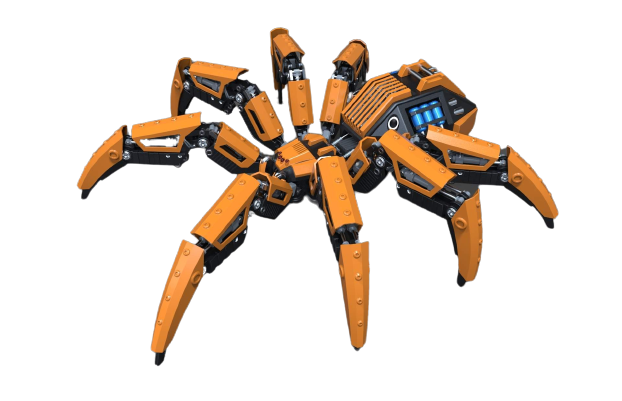
\includegraphics[width=0.5\textwidth]{./images/Chapter1/Spider2}	
	\caption[ربات عنکبوتی]{ربات عنکبوتی \cite{SpiderRobot}}
	\label{ربات عنکبوتی}
\end{figure}
\noindent
\unskip
در این پروژه، به بررسی ربات‌ عنکبوتی چهارپا می‌پردازیم که با تشکیل یک ساختار چهارپا و مکانیزم‌های تحرک پیچیده، قادر به مسیریابی و انجام وظایف متنوع در محیط‌ آزمایشگاهی می‌باشد.

\subsubsection{پایداری استاتیکی}

یک ربات با پایداری استاتیک تعادل خوبی دارد و در هنگام ایستادن به زمین نمی‌خورد. این بدین معنی است که مرکز ثقل ربات درون پایه تماس با زمین قرار دارد. فرض کنید یک ربات سه پا داریم که پاها به صورت مثلت تنظیم شده‌اند. این ربات تا زمانی‌که مرکز ثقل داخل مثلت قرار دارد، به هیچ نوع جابجایی برای ثابت ایستادن نیاز ندارد. این مثلث را «چند‌ضلعی حمایتی» می‌نامند که ناحیه‌ای افقی بالای مکان مرکز ثقل است تا پایداری استاتیک به دست آید. اگر جملات قبلی نامفهوم هستند، فقط کافی است متوجه شوید که چندضلعی حمایتی همان سطحی است که ربات روی آن ایستاده و درون نقاط حمایتی قرار دارد.

\begin{figure}[H]
	\centering
	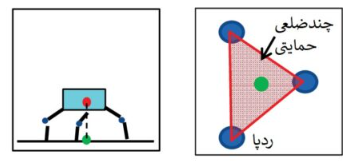
\includegraphics[width=0.5\textwidth]{./images/Chapter1/StaticStability}	
	\caption[پایداری استاتیکی]{چندضلعی حمایتی \cite{StaticStability}}
	\label{پایداری استاتیکی}
\end{figure}
\noindent
\unskip



\subsection{ربات‌های عنکبوتی چهارپا}
ربات‌های عنکبوتی چهارپا
\noindent\unskip\LTRfootnote{Quadruped Spider Robots}
، با شباهت به حرکت عنکبوت‌های طبیعی، به کمک چهار پا محرک تحرک کرده و قادر به تغییر شکل در محیط‌های مختلف هستند. این انعطاف‌پذیری در حرکت، به ربات‌ها امکان حرکت در مسیرهای مختلف، شکل گیری برای عبور از موانع و تطابق با محیط را می‌دهد. علاوه بر این، استفاده از حسگرهای چندگانه مانند دوربین‌ها، ژیروسکوپ‌ها و... به ربات‌ها امکان مشاهده و تجزیه و تحلیل محیط را می‌دهد. این قابلیت‌ها به عنوان اصول مهم در ناوبری، پیمایش محیط و انجام وظایف متنوع در برنامه‌ریزی و کنترل ربات‌های عنکبوتی چهارپا مورد استفاده قرار می‌گیرد.
برای درک بهتر یک نمونه از ربات‌های عنکبوتی چهارپا که در واقع همان ربات پایان‌نامه پیش روست و طراحی اولیه آن در محیط سالیدورک انجام شده‌است، در شکل 
\ref{نسخه‌اولیه }
قابل مشاهده می‌باشد.

\begin{figure}[H]
	\centering
	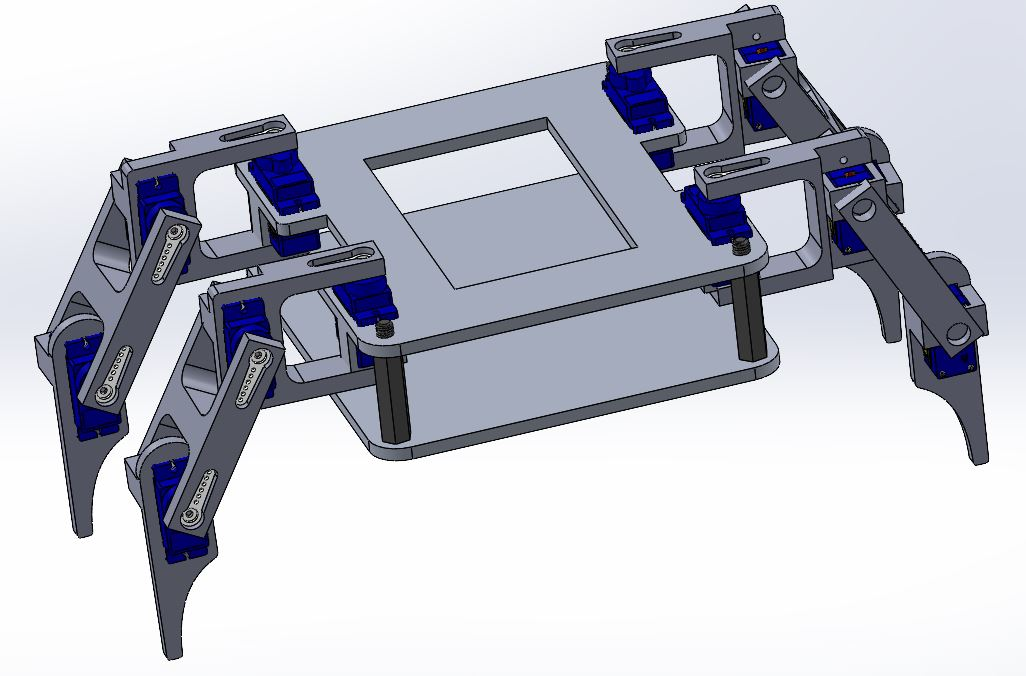
\includegraphics[width=0.6\textwidth]{./images/Chapter1/Robot_Final}	
	\caption[نسخه‌اولیه طراحی شده]{نسخه‌اولیه طراحی شده}
	\label{نسخه‌اولیه }
\end{figure}
\noindent
\unskip

\section{تاثیر هوش مصنوعی بر رباتیک}

در دهه‌های اخیر، پیشرفت‌های چشمگیری در زمینه هوش مصنوعی و رباتیک ایجاد شده است که به‌طور گسترده تأثیرات قابل‌توجهی را در صنعت و علم رباتیک ایجاد کرده است. هوش مصنوعی به عنوان یکی از شاخه‌های علوم کامپیوتر که در تلاش برای تجسم و شبیه‌سازی هوش انسانی بوده و همچنین توانایی یادگیری و تصمیم‌گیری در ماشین‌ها را دارد.

ترکیب هوش مصنوعی با رباتیک، باعث پدیدآمدن ربات‌های هوشمند و تعاملی شده است که توانایی‌هایی انسان‌نمایانه از جمله تشخیص محیط، پردازش اطلاعات، تصمیم‌گیری و انجام وظایف پیچیده را اجرا می‌کنند. این ترکیب موجب ایجاد امکانات جدید در زمینه‌های مختلف مانند صنعت، پزشکی، کشاورزی هوشمند، خودروهای خودران و بسیاری دیگر شده‌است.

در این پایان‌نامه به بررسی اثرات هوش مصنوعی بر رباتیک در یک نمونه خاص از ربات‌ها (ربات چهارپا) و همچنین کاربردها و چالش‌های متنوعی که این ترکیب مهارت‌ها ایجاد می‌کنند، پرداخته خواهد شد. این نمونه خاص‌ از ربات‌ها مثال خوبی از تعامل موثر هوش مصنوعی و روباتیک در مختلف زمینه‌ها می‌پردازد.

\section{مروری بر الگوریتم‌های مسیریابی}\label{مروری بر الگوریتم‌های مسیریابی}

امروزه با ساخت ربات‌های مختلف، برنامه مساله‌ریزی مسیر ربات، بسیار
مورد توجه قرار گرفته است. به طور خلاصه، مساله برنامه‌ریزی مسیر،
یافتن مسیری است که ربات را از نقطه شروع به نقطه هدف هدایت
می‌کند.
\cite{}
در بسیاری از کاربردها برای اینکه ربات بتواند وظیفه خود را
بدرستی انجام دهد، نیاز به حرکت در محیط دارد. الزام حرکت در محیط موجب پرسیدن این سوال می‌شود که، ربات برای انجام وظیفه خود چه مسیری را طی کند که علاوه بر ایمن بودن آن، با کمترین هزینه به هدف خود برسد. با توجه به محدودیت انرژی، تسریع در انجام کارها و عدم
برخورد ربات با موانع موجود در محیط، اهمیت این سوال بهتر درک می‌شود. پاسخگویی به این پرسش، که پرسش اساسی در زمینه تحقیقاتی مهمی تحت عنوان برنامه‌ریزی مسیر است، از دیدگاه‌های مختلف صورت گرفته است.

رویکردهای حل برنامه مسئله ریزی مسیر را می‌توان به چند دسته کلی تقسیم کرد:
\begin{enumerate}
	\item
	بلادرنگ: اگر ربات از وقایع محیطی، مکان و حرکت موانع، از قبل اطلاع نداشته باشد، آنگاه به یافتن مسیری ایمن به سوی هدف مبادرت کند، در این حالت برنامه‌ریزی بلادرنگ نامیده می‌شود.
	\cite{}
	\item
	کامل و کامل احتمالاتی: ارائه یک مسیر، در صورت وجود، کامل بودن
	الگوریتم نامیده می‌شود. کامل بودن احتمالاتی نیز به این معنی است که اگر الگوریتم تا زمان طولانی اجرا شود، در صورت وجود یک مسیر، آن را خواهد یافت.
	\cite{}
	
\end{enumerate}

از جمله روش‌های مطرح برای حل برنامه مساله‌ریزی مسیر،
الگوریتم‌های مبتنی برنمونه‌گیری هستند. در این روش‌ها با نمونه‌برداری از فضای پیکربندی، به ساخت درختی از نقطه شروع، مبادرت می شود. با رسیدن یکی از شاخه‌های درخت به نقطه هدف الگوریتم خاتمه می یابد.
 این روش در ابتدا توسط
\lr{Lavalle}
در سال 1991 تحت عنوان درخت جستجوی سریع تصادفی
\lr{RRT}
مطرح گردید.
% \section{برنامه ریزی مسیر}
% \subsection{تاریخچه برنامه ریزی مسیر}

% در این بخش به تاریخچه برنامه‌ریزی مسیر می‌پردازم.
% \subsection{مفهوم برنامه ریزی مسیر}

% در این بخش به مفهوم برنامه‌ریزی مسیر می‌پردازم.


\section{اهداف و نوآوری}

با نگاهی به پژوهش هاي انجام شده در زمينه ربات هاي عنکبوتی چهارپا مشاهده می‌شود كه در اكثر پژوهش هاي صورت گرفته به ديدگاه تئوري بيشتر اهمیت داده شده‌است. از این رو در پژوهش پيش رو تلاش شده است تا جنبه‌های عملی ربات‌‌های پادار مورد توجه قرار گرفته و همچنین تمرکز بر روی بهبود عملکرد و افزایش قابلیت‌های آنها گردد. در نتیجه این هدف، با انتخاب مکانیزمی سهل‌تر برای حرکت در محیط، به انجام وظایف محوله توسط ربات پرداخته شده‌است.
از مهمترین نوآوری این پژوهش، می‌توان به موارد زیر اشاره کرد:
\begin{itemize}
	\item
	افزودن دوربین به ربات به منظور تشخیص موانع مختلف موجود در محیط
	\item
	مانیتورینگ بلادرنگ
	\noindent\unskip\LTRfootnote{Real Time}
	تصویر محیط
	\item
	مدیریت برخط
	\noindent\unskip\LTRfootnote{Online}
	اطلاعات ارسالی از محیط به ربات و بالعکس
\end{itemize}

% اطلاعات ارسالی بر روی سرور می‌باشد.

\section{ساختار پایان نامه}

پس از اتمام پایان نامه روند هر بخش را مختصرا توضیح خواهم داد.
\newpage
\section{جمع بندی}

با توجه به طراحی اولیه برای ربات و بررسی قابلیت‌های قابل ارتقا، تمرکز اصلی بر روی بهبود مداوم و حداکثری ربات (از لحاظ نکات طراحی و ساخت و همچنین بخش نرم‌افزاری آن)در طی مراحل مختلف قرار گرفت. در نهایت با ساخت نمونه اولیه و اسمبل
\noindent\unskip\LTRfootnote{Assemble}
شدن آن به شروع جدی‌تر بخش نرم‌افزار و برطرف کردن چالش‌های عملی آن پرداخته شد.
نمونه اسمبل شده اولیه ربات در شکل
\ref{نسخه‌اسمبل شده}
قابل مشاهده می‌باشد.

\begin{figure}[H]
	\centering
	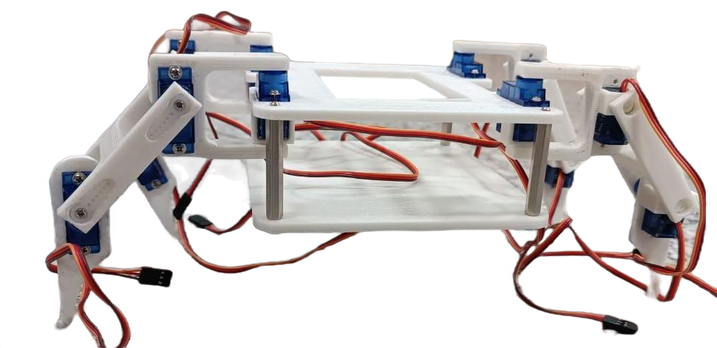
\includegraphics[width=0.5\textwidth]{./images/Chapter1/Assembled_Robot_without_background}	
	\caption[نسخه‌اسمبل شده]{نسخه‌اسمبل شده}
	\label{نسخه‌اسمبل شده}
\end{figure}
\noindent
\unskip
